\section{Model systemu}
Gra została zaimplementowana w architekturze klient-serwer. W naszym projekcie klient odpowiada jedynie za wysyłanie żądań do serwera i rysowanie na ekranie, nie jest odpowiedzialny w żadnym stopniu za obliczenia stanu gry. Taki sposób komunikacji całkowicie rozwiązał problem synchronizacji poszczególnych klatek ekranu rozsyłanych do graczy. Serwer natomiast odpowiedzialny jest za przechowywanie stanu gry, obliczenia oraz autoryzację i rejestracje użytkowników. Na rysunku \ref{fig:ddiag} przedstawiono diagram wdrożeń zaimplementowanego systemu.

\begin{figure}[ht]
    \centering
    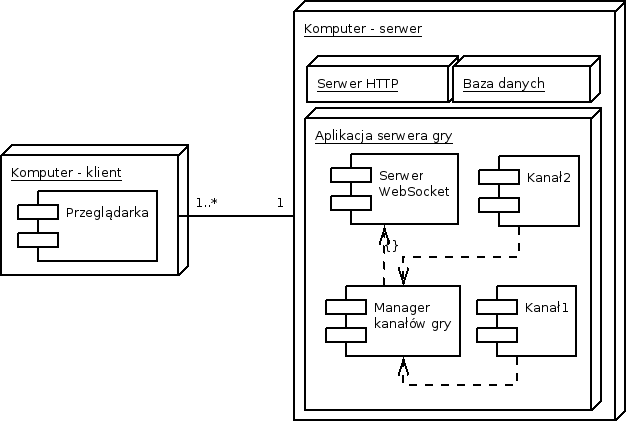
\includegraphics[scale=0.5]{imgs/ddiagram.png}
    \caption{Diagram wdrożeń zaimplementowanego systemu.}
    \label{fig:ddiag}
\end{figure}

Gracz chcący rozpocząć grę w pierwszej kolejności musi udać się pod adres \emph{www} gdzie została umieszczona część kliencka. Interfejs użytkownika pobrany zostanie tylko raz, wszelkie akcje jakie wywołuje użytkownik działają w stu procentach asynchronicznie, nie ma żadnej potrzeby aby odświeżać stronę.

Interfejs użytkownika, poprosi o podanie hasła i nazwy użytkownika w celu uwierzytelniania i przyznania dostępu do gry. Po wybraniu odpowiedniego przycisku przeglądarka połączy się oraz wyśle odpowiedni komunikat do serwera WebSocket z danymi logowania. Jeżeli dane są niepoprawne, serwer zwróci błąd a w przypadku powodzenia, aplikacja przeniesie nas to części dostępnej dla zalogowanych użytkowników.

Po udanym logowaniu serwer zwróci unikalny identyfikator sesji który będzie identyfikował zapytania przesłane od użytkownika. Klient chcący rozpocząć rozgrywkę może dołączyć do istniejącego kanału lub utworzyć własny.

Kanały utworzone na serwerze są zarządzane przez manager kanałów (\emph{channel manager}), który jest głównym punktem wejścia/wyjścia wszystkich komunikatów.

Klient, który dołączył do danej rozgrywki, na bieżąco przesyła wszystkie wydarzenia klawiatury jakie zostaną wygenerowane przez użytkownika, oraz rysuje na ekranie odebrany stan gry.
